\documentclass[a4paper,openright,openany,12pt]{book}
%\renewcommand{\baselinestretch}{1.5} % interlineado 1,5
 \usepackage{setspace}
%\doublespacing
%\onehalfspace
%\singlespace
\spacing{1.5} % espaciado

\usepackage[T1]{fontenc}
\usepackage[spanish]{babel}
\usepackage[utf8]{inputenc}
\usepackage{lmodern}

\usepackage[hidelinks]{hyperref}
\usepackage{chapterbib}
\usepackage{graphicx} % graficos
\usepackage{apacite}
\usepackage{natbib}
\usepackage{wrapfig}
\usepackage{listings} % para agregar coloreado al codigo fuente

\begin{document}
\author{valentin Basel}
\title{Robótica y educación popular}

\begin{titlepage}

\begin{center}
\vspace*{-1in}
\begin{figure}[htb]
\begin{center}

\includegraphics[width=8cm]{./figuras/utn_logo.jpg}
\end{center}
\end{figure}

Universidad Tecnologica Nacional\\
\vspace*{0.15in}
Escuela de Posgrado \\
\vspace*{0.6in}
%\begin{large}
Trabajo final de la carrera de licenciatura en tecnología educativa.\\
%\end{large}
\vspace*{0.2in}
\begin{Large}
\textbf{Proyecto de transferencia de tecnología educativa.}
%\textbf{Robótica diseñada con software y hardware libre como recurso educativo para la enseñanza de lenguajes formales.} \\
\end{Large}
\vspace*{0.3in}
\begin{large}

Implementar robótica diseñada con software y hardware libre como recurso educativo para la enseñanza de lenguajes formales.

%A Thesis submitted by Amy Wong for the degree of Doctor of Philosophy in the Mars University\\
\end{large}
\vspace*{0.3in}
\rule{80mm}{0.1mm}\\
\vspace*{0.1in}
\begin{large}
%Supervised by: \\
%Hubert J. Farnsworth \\
Valentin Basel.
\end{large}
\end{center}

\end{titlepage}
% pagina nueva (que no esta numerada)
\newpage
$\ $
\thispagestyle{empty} % para que no se numere esta pagina

%% Dedicatoria
\chapter*{}
%\pagenumbering{Roman} % para comenzar la numeracion de paginas en numeros romanos
\begin{flushright}
\textit{Dedicado a \\
bla bla}
\end{flushright}

\tableofcontents % indice de contenidos
\newpage

\section{Introducción}

Por la creciente importancia que la tecnología digital tiene hoy en día y gracias a su transversalidad en la vida cotidiana, las TIC se han vuelto una parte integral del proceso educativo. El uso de dispositivos electrónicos en el aula es una realidad y por consiguiente, la implementación y el desarrollo de propuestas educativas que permitan la evolución cognitiva de los discentes y un aprovechamiento de las nuevas tecnologías se vuelven de especial interés por sus ventajas como recurso educativo. En consecuencia, y como dice \citet{chavarria_software_2011}, la discusión sobre el uso de software y hardware libre como herramienta educativa, se vuelve trascendental para lograr el desarrollo de conceptos como la soberanía tecnológica dentro del aula.

La robótica utilizada en el  contexto educativo tiene múltiples  aplicaciones para ser aprovechada como herramienta transversal para el aprendizaje de conceptos de matemática, física y lenguajes de programación. Tomando al construccionismo de \citet{papert_childrens_1993} como teoría pedagógica central, podemos decir que la robótica es una herramienta construccionista, la cual permite a los discentes, abordar  la construcción de su propio conocimiento en base de diseñar y fabricar un robot de carácter pedagógico.  

Su carácter multidisciplinario permite abordar distintas etapas de la construcción del conocimiento por parte de los discentes, ademas de poder ser aplicada en una gran variedad temáticas, y su “espectacularidad” (entendida como la capacidad de generar algún tipo de asombro en la población estudiantil), ayuda a los docentes en la tarea de impartir la curricula planteada en el curso.

Sin embargo, la gran dificultad técnica y la cantidad de conocimientos específicos necesarios para desarrollar un robot (como electrónica, mecánica y ciencias computacionales) , ademas de un costo generalmente elevado de los kits que se consiguen en el mercado, hace que la enseñanza de robótica en las escuelas, este relegada generalmente a colegios que pueden financiar los costes de capacitación y adquisición de estos kits comerciales.

El proyecto ICARO busca desarrollar una solución técnica basada en hardware de especificaciones abiertas y software libre para facilitar la labor del docente a la hora de trabajar los contenidos técnicos complejos que implica el abordaje de una disciplina como la robótica, y ademas abaratar costos, al ser ICARO un proyecto pensado para poder implementarse en pequeña escala, sin equipamiento industrial y con la idea de que los docentes y discentes desarrollen (pensando la producción como el hecho de soldar los componentes electrónicos ) el hardware ICARO, poniendo un fuerte énfasis en la fabricación como una herramienta construccionista y de aprehensión, entendiendo esta practica como una ''herramienta de liberación'' en el sentido planteado por Paulo \citet{freire_pedagogioprimido._2015}.

Por consiguiente, La presente tesis propone un proyecto de transferencia educativo-tecnológico, basado en el diseño y desarrollo de hardware electrónico para el desarrollo de elementos de robótica, domotica o automatización, y software de control para dicho hardware, basado en los principios de soberanía tecnológica y las licencias de software libre (versión GPLV3).


\chapter{Marco Teórico}

\section{Introducción}

Abordar un proyecto de robótica como Recurso Educativo Abierto (REA/OER), implica una serie de desarrollos conceptuales y teóricos que van a mas allá del diseño y desarrollo técnico de hardware y software. El uso de REA/OER \citep{montoya2012recursos} implica un compromiso político-epistemológico con respecto al uso de la tecnología, esto es; la apropiación de términos conceptuales como ''software libre'', ''soberanía tecnológica'' y cultura libre. En lo que sigue, se da cuenta de los conceptos técnicos/teóricos para  la implementación de un proyecto de robótica educativa basado en software y hardware libre.

\section{Construccionismo}

El construccionismo es una teoría del aprendizaje diseñada por \cite{seymour_papert_desafio_1987} donde se resalta la importancia de la acción como parte principal en el proceso de aprendizaje. Toma como inspiración las ideas de la psicología constructivista, en especial el supuesto de que el conocimiento debe ser construido por el propio sujeto, el cual aprende a través de la acción. Por lo tanto, el conocimineto no es algo que se pueda solamente ''transmitir''.

\begin{wrapfigure}{r}{0.5\textwidth}
  \begin{center}
    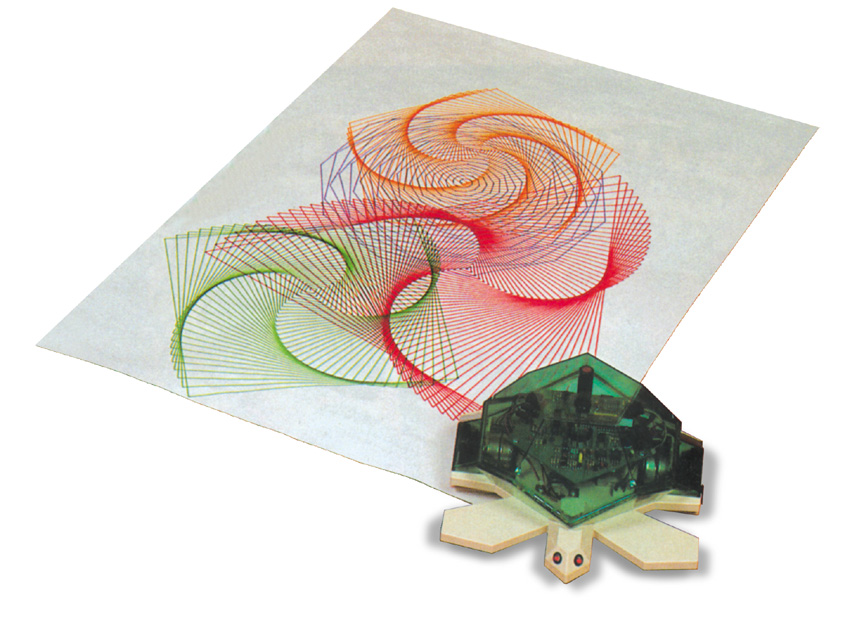
\includegraphics[width=0.2\textwidth]{figuras/Turtle_draw.jpg}
    \caption[Caption for LOF]{robot ''tortuga'' de la empresa Valiant}
    
    \label{fig:turtle }
  \end{center}
\end{wrapfigure}

% \footnote{By Valiant Technology Ltd., CC BY-SA 3.0, https://commons.wikimedia.org/w/index.php?curid=19501049}

La  teoría  del  construccionismo  afirma  que  el  aprendizaje  es  mucho  mejor  cuando  los  sujetos  se
comprometen en la construcción de un producto significativo para ellos, como podría ser un programa de computación, un robot, un juguete o una canción.

De esta forma, esta teoria involucra dos tipos de construcción: cuando los sujetos construyen
cosas en el mundo externo, simultáneamente construyen conocimiento al interior de sus mentes.  Este
nuevo  conocimiento  entonces  les  permite  construir  cosas  mucho  más  sofisticadas  en  el  mundo
externo, lo que genera más conocimiento, y así sucesivamente en un ciclo autoreforzante.

\cite{seymour_papert_desafio_1987}  da el ejemplo de los ''engranajes'' que tanto lo fascinaron en su infancia para plantear cómo pensar en un ''objeto con el cual pensar'' y ''pensarse como un engranaje'' le permitió aprender los conceptos formales matemáticos implicados en el desarrollo de un sistema de engranajes (relación entre dientes y fuerza en un tren de engranajes por ejemplo).

La propuesta central del construccionismo radica en plantear actividades de confección y construcción de artefactos aunque no necesariamente artefactos físicos. Estos, funcionan como facilitadores del aprendizaje porque los sujetos, al construir un dispositivo (un robot, un castillo o un programa de computadora), construyen también sus propias estructuras de conocimiento. Papert afirma que los sujetos además, deben construir objetos que sean de su interés personal, para poder interesarse mas en el proceso de construcción (y por ende, en su proceso de construcción de conocimiento). Al mismo tiempo, los objetos construidos ofrecen la posibilidad de hacer más concretos, palpables y visibles (dentro del esquema de pensamiento del sujeto) los conceptos abstractos o teóricos, y por tanto, hacerlos más fácilmente comprensibles.



\section{Ciencias de la computación}

Tomando como referencia a la propuesta de la fundación \cite{sadosky2013cc} podemos hacer una diferencia entre las  tecnologías de la  información y comunicación (TIC) y las ciencias de la computación (CC), donde las primeras (TICs) se refieren a nivel global sobre el uso de herramientas basadas en computadoras (ofimáticas, navegación por internet por ejemplo), mientras que las ciencias de la computación están orientadas específicamente a la generación de habilidades y competencias especificas 

\section{Lenguajes formales}

Un lenguaje formal es un lenguaje cuyos símbolos (alfabeto) y reglas para unir esos símbolos (gramática) están formalmente definidos \citep{giro_lenguaje_2015}.

Un lenguaje de programación es un lenguaje formal, como la lógica y la matemática, con la diferencia que fue diseñado para realizar procesos que pueden ser llevados a cabo por computadoras. Entre sus características principales, se encuentra la posibilidad de poder crear programas que gobiernen el comportamiento de una computadora, tanto a nivel físico (hardware) como lógico (software).

Durante la decada del cincuenta, en la primera época de las computadoras (las grandes mainframes como la ENIAC), estas eran programadas directamente escribiendo ''ceros y unos'' sobre su memoria, utilizando lo que se define como \textbf{lenguaje de máquina}, o una serie de reglas nmemo-técnicas llamadas \textbf{lenguaje ensamblador}. La dificultad de programar software cada vez más complejo, hizo que se desarrollaran lenguajes de programación cada vez más alejados del lenguaje de maquina y mas cercanos al lenguaje natural. Se dice comúnmente que un lenguaje de bajo nivel es aquel que se asemeja a la forma de trabajar de una computadora (assembler, por ejemplo), y que un lenguaje de alto nivel trata de ser mas parecido al lenguaje que usamos los seres humanos (python, por ejemplo); por lo tanto, es más fácil de entender para los programadores y para impartir cursos de iniciación a la programación \citep{de2016introduccion}.

\subsection{Python}


\begin{wrapfigure}{r}{0.5\textwidth}
  \begin{center}
    
\includegraphics[width=0.2\textwidth]{figuras/Python-logo.png}
    \caption[Caption for LOF]{Logotipo de python}
    
    \label{fig:python_logo}
  \end{center}
\end{wrapfigure}

Python es un lenguaje de programación interpretado, de alto nivel y multi paradigma, cuya filosofía hace hincapié en una sintaxis que favorezca un código fácil de leer para los programadores.Como dice \cite{marzal2003aprender}, python es un lenguaje ideal para la enseñanza de programación porque tiene una \textit{sintaxis} que facilita la economía de símbolos auxiliares (como el símbolo '';'' usado para indicar el final de linea en lenguaje C), es \textit{expresivo} (entendiendo esto como su capacidad para decir mucho con pocas lineas de código), y su \textit{semántica} es elegante, haciendo que sea fácil de entender y escribir.

Entre sus características \citep[pág 15]{marzal2004introduccion} están: 

\begin{itemize}
  \item Python es un lenguaje muy expresivo, es decir, los programas Python son muy compactos.
  \item Python es muy legible. La sintaxis de Python es muy elegante y de fácil lectura.
  \item Python ofrece un entorno interactivo que facilita la realización de pruebas.
  \item Python puede usarse como lenguaje imperativo procedimental o como lenguaje orientado a objetos.
  \item Posee un rico juego de estructuras de datos que se pueden manipular de modo sencillo.
 
\end{itemize}

\section{Soberanía tecnológica}

El concepto de soberanía tecnológica plantea una alternativa al proceso calificado por James \citet{boyle_second_2003} como el “segundo cercamiento de los bienes comunes”. Si la acumulación inicial del capital se produjo mediante el cerco (enclosure) de las tierras comunales, este segundo cerco a los bienes comunes pretende la apropiación privada, mediante el sistema de marcas registradas, patentes y las leyes de propiedad intelectual, de objetos e ideas que hasta ahora quedaban excluidos por considerarse bienes comunes inapropiables. En este contexto, el uso de software libre sirve como herramienta que puede ser utilizada -como se propone en el presente proyecto- para lograr, siguiendo a Paulo \citet{freire_pedagogiautonomi:_2006}, una “pedagogía de la autonomía”. Y no solo una base de usuarios cautivos para las empresas desarrolladoras de software. 

\section{Software libre}

El software libre es un movimiento que comenzó en el año 1983 cuando Richard \cite{stallman_software_2007} anunció el proyecto GNU en contra posición a la aparición de monopolios artificiales en el desarrollo de software \citep{beatriz_busaniche_argentina_2010}. Se podría decir que la meta del movimiento fue dar libertad a los usuarios de programas de computadoras remplazando el software con términos de licencias restrictivas (software privativo)  por una alternativa libre.

La comunidad de desarrolladores de software libre plantea que el software, para ser considerado libre, debe poder ser copiado, estudiado, distribuido y modificado libremente por cualquier persona o comunidad. En este sentido, se vuelve de vital importancia contar con el código fuente (y no sólo el código maquina o binario) de los programas para poder estudiarlos y modificarlos; además de tener una licencia (la licencia GNU/GPL) que proteja el derecho de autor y permita que ese código pueda ser distribuido sin el peligro de que sea apropiado por alguien más.

Por lo tanto para poder entender el concepto del software libre y las implicancias políticas del movimiento, lo principal es analizar los conceptos técnicos del desarrollo de software y la diferencia entre el código binario (archivo ejecutable)  y el código fuente (escrito en un lenguaje de programación).

\subsection{Código fuente}

El software que diariamente usamos en nuestras computadoras esta compuesto por archivos  binarios, largas listas de ceros y unos (código binario) con los cuales la computadora lee y ejecuta las instrucciones que estos archivos les brindan. Originalmente, en el desarrollo de software, los ingenieros escribían directamente sobre la memoria de las computadoras de la época, grandes mainsframes que ocupaban habitaciones completas. Con el crecimiento de la potencia de las computadoras, y la consiguiente complejidad en el desarrollo  los programas necesarios para controlar estas nuevas máquinas, se comenzó a ver la necesidad de contar con una forma más eficiente y sencilla de crear dichos programas. Es en esta época que nace la idea un programa compilador que convierta la información escrita en un lenguaje formal (con cierto grado de aproximación a un lenguaje natural humano) y la pase a un lenguaje de máquina (código binario).

Un compilador es, en su definición mas genérica, un programa que toma como entrada un texto escrito en cierto lenguaje y produce como salida otro texto en un lenguaje diferente \citep{grune_diseno_2007}, manteniendo el archivo original (código fuente) y el archivo de salida (código objeto, generalmente un archivo binario ejecutable por la computadora). Es decir que un compilador convierte  o traduce (como término más general) un archivo de código fuente a un archivo de código binario, permitiendo escribir en un lenguaje más parecido al lenguaje natural (y, por tanto, más sencillo de entender para los humanos).

   Por consiguiente, podemos considerar al lenguaje de programación como un lenguaje formal, donde una serie de instrucciones inequívocas conforman un algoritmo \citep{giro_lenguaje_2015}  que puede ser convertido por un compilador en un archivo de instrucciones binarias para ser ejecutado por una computadora.
   
Richard \cite{stallman_software_2007} realiza la analogía entre el código fuente y una receta de cocina (los pasos para hacer una torta por ejemplo), donde siguiendo instrucciones sencillas y no ambiguas se obtiene un producto final (la torta en este caso). En este esquema, la receta de cocina sería igual al código fuente, y el producto final al código binario (o ejecutable). Naturalmente, si nosotros sólo tenemos la torta, descubrir como obtener de vuelta la receta (ingeniería inversa) es mucho más difícil que en sentido inverso (receta-torta).

Para ejemplificar concretamente, en la siguiente tabla podemos ver las diferencias entre el software y el código fuente propuesta por \cite{hart_open_2003}.

\begin{table}
\begin{center}
\begin{tabular*}{1\textwidth}{@{\extracolsep{\fill}} | l | l | } 
\hline
Lenguaje de programación & Código fuente  \\ \hline
ANSI C &
\begin{lstlisting}[language=C]
#include <stdio.h>
int main(int argc, char* argv[])
{
puts("Hola mundo!");
}
\end{lstlisting}
\\ \hline
Python &
\begin{lstlisting}[language=PYTHON]
print "hello world"
exit()
\end{lstlisting}
\\ \hline
binario                          & 01001000011001010110110001 \\
(''hello world'' en ASCII)       & 10110001101111001000000101 \\
                                 & 01110110111101110010011011 \\
                                 & 0001100100 \\ \hline
\end{tabular*}
\label{cod_fuente}
\caption{Lenguajes de programación, comparación entre código fuente y código máquina}
\end{center}
\end{table}

  
  
Como plantean Jordi \cite{adell_software_2007}, cambiar un programa escrito en python, por ejemplo, para que en lugar de decir “Hello World” diga “Hola Mundo” sería bastante trivial y fácil de hacer. Sin embargo, hacerlo desde código binario se vuelve muy complejo, y eso que solamente son los caracteres de la palabra “Hello World” y no un programa completo, el cual hasta el más sencillo, puede contener miles y hasta  millones de ceros y unos.

 Por tanto, para un programador es necesario contar con el código fuente de un software para poder modificarlo, estudiarlo y comprender su funcionamiento (y que no sea solamente una caja negra).
 
Teniendo en cuenta los conceptos mencionados, podemos explicar algunas de las definiciones que se utilizan para que un software sea considerado como software libre. Richard \cite{stallman_software_2007} define cuatro “libertades” que tiene que tener el software para considerarlo libre:

\begin{itemize}
   \item libertad 0: La libertad de usar el programa, con cualquier propósito (Uso)
   \item libertad 1: La libertad de estudiar cómo funciona el programa y modificarlo, adaptándolo a las propias necesidades (Estudio).
   \item libertad 2: La libertad de distribuir copias del programa, con lo cual se puede ayudar a otros usuarios (Distribución).
   \item libertad 3: La libertad de mejorar el programa y hacer públicas esas mejoras a los demás, de modo que toda la comunidad se beneficie (Mejora).
 \end{itemize} 
 
Un programa es software libre si otorga a los usuarios todas estas libertades de manera adecuada. Por lo tanto, el echo de contar con el código fuente es una condición necesaria para poder ejercer las cuatro libertades que plantea la FSF (Free Software Foundation). Lo dicho hasta aquí supone que todos los programas desarrollados y distribuidos bajo licencias libres (por ej. -la licencia GNU/GPL V3) tienen que se distribuidos con los archivos de código fuente además de de los archivos ejecutables (en el caso de programas compilados).

\begin{wrapfigure}{R}{0.5\textwidth}
%\begin{figure}[h]
  \begin{center}
    
\includegraphics[width=0.5\textwidth]{figuras/fsf.png}
    \caption{Logotipo del Free Software Foundation}
    \label{fig: }
  \end{center}
%\end{figure}
\end{wrapfigure}

El software libre busca proteger las libertades individuales de los usuarios de computadoras como oposición a los desarrollos de software privativos (como los define la FSF), licencias restrictivas de uso, software malicioso (malwares, backtrack) monopolios \citep{beatriz_busaniche_argentina_2010}, y prácticas poco éticas que algunas empresas pueden aplicar a sus usuarios. En cambio, gracias al software libre, los usuarios no están restringidos por el desarrollador de la aplicación y son dueños completos del programa que necesitan usar, permitiendo a comunidades, organismos estatales y/o universidades, adaptar dicho software a las necesidades concretas de cada grupo, y así poder dar respuesta a necesidades puntuales que podrían no ser ''rentables'' para una empresa particular.

El software libre es un desarrollo soportado por las comunidades y para las comunidades, donde el esquema de desarrollo es distribuido y global, o como dice \citep{raymond_catedral_1998} un esquema dónde el desarrollo de software libre es más parecido a un ''bazar'' dónde todos aportan de manera ''desorganizada'' y des centralizada, en contra posición a un desarrollo más parecido a una ''catedral'', dónde un arquitecto es el jefe central del desarrollo, en un esquema fuertemente estructurado.

\section{Hardware de especificaciones abiertas }

\begin{wrapfigure}{r}{0.5\textwidth}
  \begin{center}
    
\includegraphics[width=0.2\textwidth]{figuras/Open-source-hardware-logo.png}
    \caption{Logotipo del Open Source Hardware}
    \label{fig: }
  \end{center}
\end{wrapfigure}

El movimiento de hardware libre (o hardware de especificaciones abiertas) , busca llevar el concepto del software libre (la libertad de usar, estudiar, distribuir o mejorar el software) al diseño de  componentes físicos, especificando una licencia que permite distribuir planos y código fuente de desarrollos de PCBs (Printed Circuit Board por sus siglas en ingles) y hardware electrónico. Asimismo, se considera que un diseño de circuito (esquemático, diseño de PCB y archivos GERBER) debe ser desarrollado con software libre y usando formatos abiertos.

De acuerdo a la declaración de principios de la \textbf{Open Source Hardware association} \footnote{http://www.oshwa.org/definition/spanish/} , podemos decir que:

\begin{center}
\textit{
Hardware de Fuentes Abiertas (OSHW en inglés) es aquel hardware cuyo diseño se hace disponible públicamente para que cualquier persona lo pueda estudiar, modificar, distribuir, materializar y vender, tanto el original como otros objetos basados en ese diseño. Las fuentes del hardware (entendidas como los ficheros fuente) habrán de estar disponibles en un formato apropiado para poder realizar modificaciones sobre ellas.
}
\end{center}


\begin{wrapfigure}{r}{0.5\textwidth}
  \begin{center}
    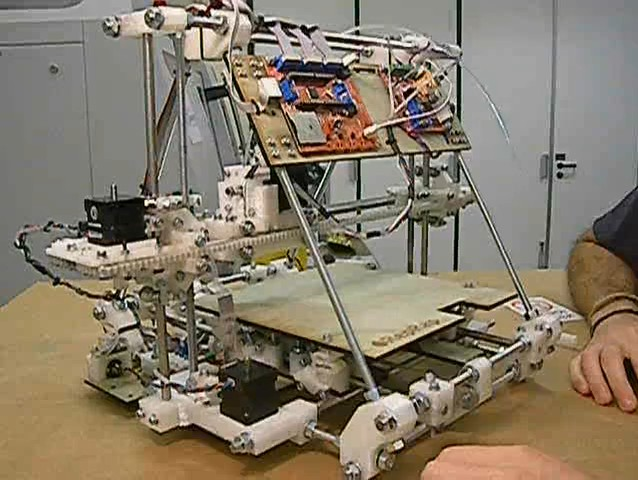
\includegraphics[width=0.5\textwidth]{figuras/reprap.jpg}
    \caption[Caption for LOF]{Impresora 3d diseñada con hardware libre}
       
    \label{fig:reprap }
  \end{center}
\end{wrapfigure}

%\footnote{By CharlesC - http://vimeo.com/6865848 - video from open-source RepRap project, CC BY-SA 3.0, https://commons.wikimedia.org/w/index.php?curid=8020149}

Idealmente, el hardware de fuentes abiertas debería ser diseñado de modo tal que puedan utilizarse en su construcción componentes, materiales y herramientas de alta disponibilidad y fácil acceso (en lo posible), empleando herramientas de fuentes abiertas (en el caso del software de desarrollo); esto permite maximizar la posibilidad de construir y usar ese hardware por parte de los usuarios. 

Es importante notar como la OSHW plantea que para que un hardware sea considerado de estándares abiertos, no sólo debe distribuirse  sus planos y esquemáticos con un formato libre. Ademas, el diseño deberia contemplar la posibilidad de fabricar ese mismo hardware por parte de los usuarios. El hardware de fuentes abiertas da libertad de controlar la tecnología y al mismo tiempo permite compartir conocimientos.

\citet{gonzalez_hardware_2003} plantean una clasificación del hardware en función de su diseño y el software empleado para su creación, definiendo una clasificación primaria de los tres tipos de archivos necesarios para la fabricación de un PCB, el \textit{esquemático},el archivo de  \textit{pcb} y el archivo \textit{GERBER}. En función de esa clasificación, se puede separar al hardware en tres tipos:

\begin{itemize}
   \item (P): Software de diseño propietario.
   \item (L): Software de diseño libre.
   \item (M): Software de diseño propietario pero multi plataforma (funciona en sistemas operativos libres y también en propietarios)
 \end{itemize} 

Por tanto los tres archivos de construcción para el circuito electrónico, pueden ser de clasificación como enteramente libres (tipo \textbf{LLL}) o completamente propietarios (\textbf{PPP}), y todas sus combinaciones posibles.


\subsection{Software libre en la escuela}

\citet{adell_software_2007} consideran al Software libre una alternativa para aplicar en el contexto del aula por sus ventajas pragmáticas (menor o hasta incluso nulo costo por licencias) que permiten ahorrar presupuesto, y por sus valores ético, políticos y sociales \citep{hart_open_2003}, que funcionan como disparadores de discusiones sobre los valores que una institución educativa tendría que promover.El software libre en la educación trata sobre la libertad de los docentes y dicentes, porque Como dice Paulo \citet{freire_pedagogioprimido._2015}: \textit{''Nadie libera a nadie, ni nadie se libera solo. Los hombres se liberan en comunión''}.

La incorporación del software libre en el desarrollo curricular del aula, promueve la cooperación entre las personas; si el software privativo la convierte en un delito \citep{adell_software_2007}, el software libre permite a las instituciones escolares sumar sus esfuerzos académicos a un proyecto global, independiente de los vaivenes económicos de las grandes corporaciones, y adaptable a las necesidades concretas de la comunidad donde ese establecimiento está asentado.

Usando software libre, los alumnos pueden disponer de copias gratuitas de los programas que necesiten para el trabajo escolar, sin restricciones de licencias que obligan a tener un software de menor calidad para presionar a los usuarios a comprar versiones ''completas''. Al disponer del código fuente, el mismo puede adaptarse a las necesidades del docente para situaciones concretas, como traducir dicho software al idioma de sus alumnos (como el caso de la traducción de la suite ofimática Libreoffice al idioma aimara\footnote{http://www.elmundo.es/navegante/2007/08/03/tecnologia/1186167876.html}). 

Los proyectos de software libre suelen tener un coste inicial de desarrollo muy bajo \citep{adell_software_2007}. Generalmente empiezan como un desarrollo personal de algún programador o pequeño grupo de entusiastas y, gracias al trabajo global y distribuido logran crecer y obtener una ''masa critica'' de desarrolladores. Como menciona \cite{boyle_second_2003}:

\begin{center}
\textit{en una red global hay tanta gente y los costos son tan bajos que incluso los proyectos relativamente complejos atraen a las personas motivadas y capaces cuyo precio base ya ha sido superado}
\end{center}

 De esa forma, proyectos muy complejos pueden ver la luz, y ese mecanismo puede ser aprovechado por los colegios para ser generadores de contenido que pueda ser aprovechado a su vez por otras instituciones.

\section{Robots}

A nivel histórico, la palabra robots ha sido definida por la obra de teatro R.U.R. (Robots Universales Rossum) del dramaturgo checo Karel Čapek; allí se usó por primera vez la expresión "robotnik" para referirse a seres humanos sintéticos creados para ser esclavos de la humanidad  \citep{zabala_robotica_2007}. Sin embargo la popularidad del término robot se debe al escritor y divulgador científico Isaac Asimov, quien usó el termino robótica para designar a la disciplina que estudia a sistemas autónomos con cierto grado de capacidad para tomar decisiones e interaccionar con su medio (físico o virtual).

\begin{wrapfigure}{r}{0.5\textwidth}
  \begin{center}
    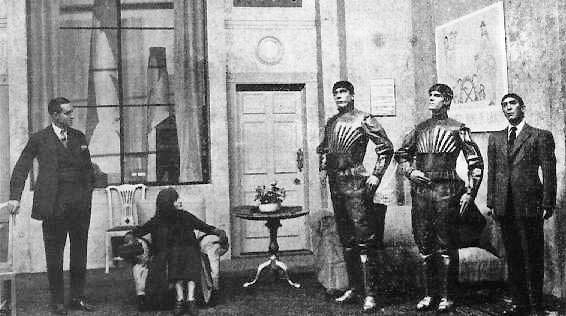
\includegraphics[width=0.5\textwidth]{figuras/Capek_play.jpg}
    \caption[Caption for LOF]{una escena de la obra de Karel Capek's R.U.R. (Rossum's Universal Robots), en donde podemos ver a los ''robots''.}
       
    \label{fig:reprap }
  \end{center}
\end{wrapfigure}

Se podría decir que cualquier sistema que posea sensores, actuadores y algún tipo de dispositivo que le permita realizar algoritmos de procesamientos, es un robot. Una definición tan laxa haría que prácticamente cualquier dispositivo pueda ser considerado un robot. Hay múltiples definiciones de la palabra robot, en función de las necesidades específicas de cada país u organización. Por ejemplo si tomamos la definición empleada por la R.I.A \footnote{https://www.robotics.org/}, un robot (sobre todo pensando en el robot industrial) es\footnote{https://definitions.uslegal.com/r/robotics/} : 
  

\begin{center}
\textit{un robot es un manipulador multifuncional y reprogramable diseñado para desplazar materiales, componentes, herramientas o dispositivos especializados por medio de movimientos programados variables con el fin de realizar tareas diversas.} [Traducción propia]
\end{center}

Por otro lado, la J.A.R.A\footnote{http://www.jara.jp/e/index.html} (Japan Robot Association, ex J.I.R.A) usa una definición menos orientada a los manipuladores industriales \citep{reyes_cortes_robotica:_2011}:

\begin{center}
\textit{Los robots son dispositivos capaces de moverse de modo flexible análogo al que poseen los organismos vivos, con o sin funciones intelectuales, permitiendo operaciones en respuesta a las órdenes humanas}
\end{center}

Como podemos ver, hay múltiples definiciones de la robótica, algunas más orientadas a la industria, y otras más generales, donde un robot puede ser desde una androide (robot con forma humanoide) hasta un electrodoméstico. 


\section{Robótica educativa}
El construccionismo de Papert promueve la utilización de computadoras como recurso para coadyuvar al desarrollo de nuevas maneras de pensar y aprender. Papert plantea que la única habilidad competitiva a largo plazo es la habilidad para aprender; su enfoque metodológico está orientado a usar las computadoras como herramientas para posibilitar ese desarrollo cognitivo en los alumnos. \citet{sanchez_robotica_2012} afirman que el construccionismo es reconocido como una teoría educativa que fundamenta el uso de la tecnología digital en educación.

En cuanto al uso de robótica como recurso educativo, \citet{sanchez_robotica_2012} resaltan que, por su carácter multidisciplinario, la robótica es una herramienta interesante como recurso facilitador del aprendizaje y el desarrollo de competencias generales. Permite trabajar transversalmente múltiples disciplinas, y sirve como motivador para que los discentes lleven a cabo proyectos mediante los cuales puedan experimentar y desarrollar sus actitudes cognitivas. En este sentido, y siguiendo a \citet{pitti_experiencias_2010}, la robótica es una herramienta construccionista. 
 
Uno de los mayores problemas de la implementación de la robótica en el aula, es la gran carga de contenido técnico que debe afrontar el docente para poder trabajar con su currícula. En consecuencia, varios fabricantes diseñaron Kits para el uso de robótica con fines educativos, sin embargo estos kits suelen ser extremadamente caros y por lo tanto restrictivos para su utilización masiva en las escuelas. El coste operativo de implementar un kit de robótica comercial puede ser prohibitivo para colegios de bajos ingresos, pero también el costo de mantenimiento (reparación y remplazo de piezas defectuosas, actualizaciones etc.) termina siendo un factor clave a la hora de usar los robots como herramientas pedagógicas, a causa del ''peligro'' de que los alumnos rompan los robots y que reponerlos salga tan caro como comprar un kit nuevo.

La Robótica educativa con software y hardware libre es una opción más viable para su aplicación en el proceso de aprendizaje, 
porque permite a las escuelas adaptar la tecnología a las necesidades especificas de la institución, permitiendo reutilizar componentes que se encuentran en el colegio ( aportados por la comunidad escolar), reciclando y  ahorrando costos. A su vez por la gran expectativa que genera en los alumnos (y docentes), y al ser de código fuente libre, permite romper barreras culturales y políticas que pueden ir en detrimento de la calidad educativa; barreras como el alto costo de adquisición de los elementos, las licencias privativas para el software de control o la falta de documentación específica para comunidades minoritarias (traducciones a idiomas que no son consideraos viables comercialmente por ejemplo). La robótica educativa con software y hardware libre permite aprovechar las ventajas que ofrece la filosofía de desarrollo que promueven las comunidades de software libre, donde ''mil ojos ven más que uno'' \citep{raymond_catedral_1998}, permite así involucrar a la comunidad escolar en su conjunto y que las soluciones aportadas por el grupo puedan ser utilizadas en otros colegios y vice-versa, generando una situaciones en las que todos los involucrados salen favorecidos.

\chapter{Estado de la cuestión}

\section{Introducción}

En este capítulo, se tratará de dar cuenta de la importancia de la la enseñanza de las ciencias de computación en la escuela media, señalando cómo la robótica puede servir de herramienta para lograr ese cometido, aprovechando sus particularidades y ventajas a la hora de abordar conceptos propios del pensamiento algorítmico (repeticiones, recursividad, saltos condicionales). Estos planteos se encuentran en consecuencia con la actual ley Nacional de Educación N\grad 26.206 que, en su artículo 30\grad, Inc. F, enuncia: 

\textit{Desarrollar  las  capacidades  necesarias  para  la  comprensión  y  utilización  inteligente  y  crítica  de  los  nuevos  lenguajes  producidos  en  el  campo  de  las tecnologías de la información y la comunicación.}

Podemos decir que las ciencias de la computación \citep[pág 4]{sadosky2013cc} se volverán de vital importancia a la hora de pensar un esquema curricular especifico para abordar los contenidos básicos propuestos por dicha ley.

\section{Antecedentes}

\subsection{Lenguaje LOGO}
El uso de dispositivos robots para enseñanza, tiene su origen en el ya referido trabajo de Seymour Papert, y su desarrollo del lenguaje LOGO. Este lenguaje formal \citep{giro_lenguaje_2015} fue diseñado para trabajar conceptos de matemáticas y geometría mediante la interacción con un robot con forma de tortuga (de ahí que el logotipo de LOGO sea una tortuga). Este dispositivo se movía sobre una superficie plana dibujando en función de las instrucciones previamente creadas en una computadora. Basado en ese esquema, los discentes programaban en lenguaje LOGO (un lenguaje muy parecido en su forma al lenguaje LISP), luego activaban el robot tortuga y la computadora enviaba las órdenes para que éste se mueva, dibujando sobre un papel. 

A través de esa experiencia, Papert colabora con la empresa LEGO para fabricar el producto LEGO\textsuperscript/LOGO, el cual después pasaría a ser conocido como LEGO MINDSTORM\textsuperscript{\texttrademark}, una plataforma física basada en fichas LEGO\textsuperscript{\textregistered} que también incluye hardware de adquisición de datos capaz de leer sensores y trabajar sobre diversos actuadores.

Con el tiempo, el lenguaje LOGO abandonaría la tortuga robot. El elevado costo de cada robot tortuga y el abaratamiento de las micro computadoras (por ej. COMMODORE\textsuperscript{\textregistered} c64) con capacidad de procesar gráficos a color  hicieron que fuera muy difícil implementar una currícula basada en LOGO solamente usando elrobot tortuga.

\begin{wrapfigure}{R}{0.5\textwidth}
  \begin{center}
    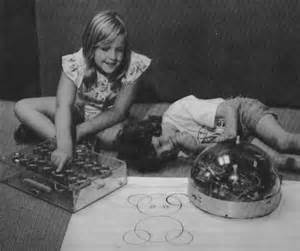
\includegraphics[width=0.5\textwidth]{figuras/logo_robot.jpg}
    \caption[Caption for LOF]{robot 'tortuga' original diseñado por el M.I.T}
    
    \label{fig:tortuga_mit}
  \end{center}
\end{wrapfigure}

El lenguaje LOGO está diseñado para ser sencillo de aprender, con instrucciones ''primitivas'' (en el argot LOGO) que son intuitivas para el usuario; la palabra 'adelante', hace que la tortuga avance N pasos,  al igual que ''atrás'' hace que retroceda. Sin embargo sigue siendo un lenguaje de programación completo y capaz de hacer lo mismo que otros lenguajes de propósito general  (como C, FORTRAN u otros lenguajes de la época). 

Una de las ventajas de LOGO es su facilidad de poder hacer ''algo'' con muy pocas lineas de código (típicamente algún dibujo con la ''tortuguita''), \cite{seymour_papert_desafio_1987} plantea que cualquier niño, bajo las condiciones adecuadas, puede aprender un lenguaje de programación como LOGO.

Originalmente, las primeras pruebas de LOGO se hicieron con robots como el de la figura \ref{fig:tortuga_mit}, el cual estaba pensado para ser robusto, y capaz de soportar hasta el peso de un niño encima. Las computadoras de la época no tenían capacidad de procesar gráficos de alta definición (y las impresoras eran caras y de uso casi exclusivo en las empresas), por lo tanto la ventaja de disponer de un robot que dibuje eran muy atractivas.

\begin{wrapfigure}{R}{0.5\textwidth}
  \begin{center}
    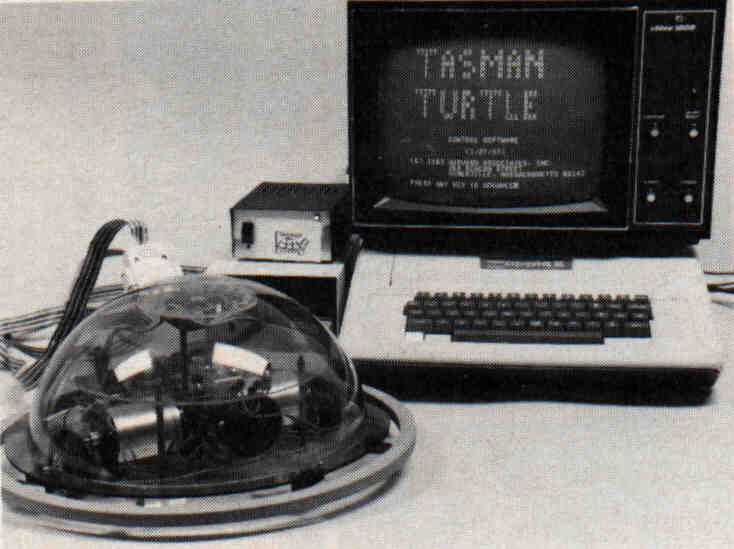
\includegraphics[width=0.5\textwidth]{figuras/turtle_with_apple.JPG}
    \caption[Caption for LOF]{Versión 'mini' del robot tortuga controlado por un micro computador Apple}
    
    \label{fig:tortuga_2}
  \end{center}
\end{wrapfigure}

Con el advenimiento de las micro computadoras (como las ZX spectrum\textsuperscript{\texttrademark}  y las commodores\textsuperscript{\texttrademark} C64), que contaban con la capacidad de trabajar  en monitores a color (o en los televisores CRT de la época) tenian bajo costo de adquisición, se dejó de utilizar a los robots tortuga, para directamente trabajar con el lenguaje de programación LOGO y una ''tortuga virtual'', menos llamativa pero mucho mas barata de adquirir para los colegios. 

\subsection{ARDUINO\textsuperscript{\texttrademark} y la revolución del hardware libre.} 


El primer modelo de la placa Arduino\textsuperscript{\texttrademark} fue introducido en 2005, ofreciendo un bajo costo y facilidad de uso para novatos y profesionales. Buscaba desarrollar proyectos interactivos con su entorno mediante el uso de actuadores y sensores. Su bajo costo y la enorme cantidad de documentación generada por las distintas comunidades de desarrolladores y entusiastas permitió que la plataforma Arduino\textsuperscript{\texttrademark} se volviera un estándar a la hora de hablar sobre automatización o IOT (Internet of things).

Actualmente los miles de kits para enseñanza de robótica que se diseñan y fabrican (a pequeña o gran escala) están basados en la arquitectura Arduino\textsuperscript{\texttrademark} y la serie de micro controladores AVR\textsuperscript{\textregistered} de 8 bits. La inmensa documentación disponible y la facilidad de adquisición de los componentes, ha expandido su uso por parte de diversas comunidades y con diversas finalidades, entre ellas, la enseñanza de robótica. Esta gran demanda,  también incidió en el abaratamiento de los costos de fabricación del hardware. Los kits generalmente constan de una serie uniforme de componentes electrónicos y mecánicos, como servo motores, motores de corriente continua, sensores analógicos / digitales y componentes de electrónica discreta (resistencias, leds, capacitores, entro otros), que permiten trabajar una serie de sistemas de automatización, robótica y/o domótica de mayor o menor complejidad.

\begin{wrapfigure}{r}{0.5\textwidth}
  \begin{center}
    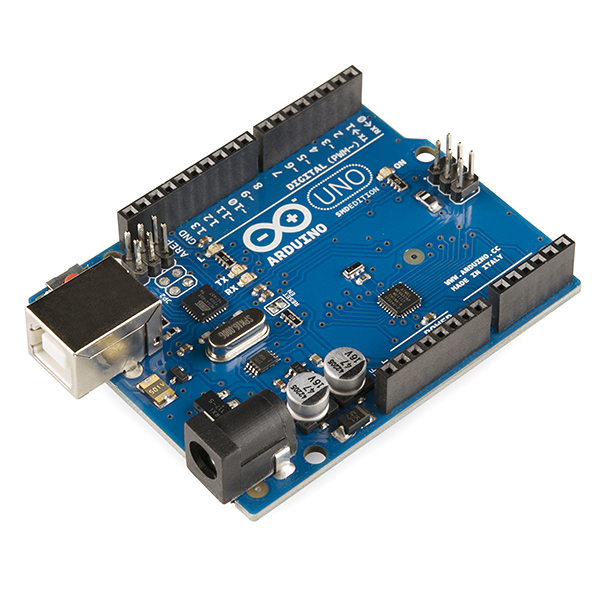
\includegraphics[width=0.5\textwidth]{figuras/Arduino_Uno_-_R3.jpg}
    \caption[Caption for LOF]{Arduino\textsuperscript{\texttrademark} Uno Rev. 3}
       
    \label{fig:arduinouno }
  \end{center}
\end{wrapfigure}

%\texttrademark : pone el símbolo TM
%\textregistered : pone el símbolo consistente en una R rodeada de un círculo
%\textcopyright : pone el símbolo consistente en una C rodeada de un círculo
\section{lenguajes de programación en la enseñanza}

En la actualidad y en el marco de la ley Nacional de educación, la enseñanza de la ciencia computacional está tomando relevancia a nivel curricular. La falta de profesionales especializados en programación y la constante demanda de ''mano de obra'' por parte de la industria del software (software factory) se ha vuelto un factor de preocupación por parte de las autoridades nacionales. Para tratar de paliar esa problemática, se están implementando distintos planes y programas gubernamentales. Dentro de estos proyectos podemos encontrar el Programa \textbf{Escuelas del Futuro}, situado en la órbita de la Secretaría de Innovación y Calidad Educativa del Ministerio de Educación y Deportes de la Nación. El mismo busca: 

\begin{center}
\textit{
crear un Proyecto con el objeto de generar un cambio transformador en las estrategias pedagógicas y políticas de contenidos para integración del sistema educativo a la cultura digital.
Que para el logro de los objetivos previstos en los considerandos precedentes, resulta conveniente la creación del Proyecto ''Escuelas del Futuro'' orientado a propiciar alfabetización digital de todos/as los/as estudiantes de la Argentina, a través de integración de áreas de conocimiento emergentes, como la programación y la robótica. \footnote{Resolución Ministerial 2.376/16 Ministerio de Educación y Deportes, consultado en http://www.saij.gob.ar/proyecto-escuelas-futuro-nv15957-2016-12-05/123456789-0abc-759-51ti-lpssedadevon?}
} 
\end{center}

Desde esa perspectiva, y como señalan desde la Fundación Sadosky, la alfabetización digital parte de la enseñanza de la ciencia computacional  pensada como un conjunto amplio de fundamentos y principios independiente de tecnologías  \citep[pág 12]{sadosky2013cc} que incluyen:

\begin{enumerate}
  \item Programación y algoritmos
  \item Estructuras de datos
  \item Arquitecturas y redes de computadoras
\end{enumerate}

La ciencia computacional permite fomentar habilidades que pueden ser aplicadas a variados campos de estudio como:

\begin{enumerate}
  \item Modelización y formalización.
  \item Descomposición en sub problemas.
  \item Generalización y abstracción de casos particulares.
  \item Proceso de diseño, implementación y prueba.
\end{enumerate}

De esta forma la enseñanza de un lenguaje formal toma una particular relevancia dentro del esquema educativo actual, que busca resolver los problemas planteados por la necesidad de alfabetizar digitalmente a la población.

Sin embargo, hay críticas concretas a la enseñanza del ''pensamiento algoritmico'' en contraposición a la enseñanza de lenguajes formales específicos. La idea de pensamiento algorítmico es que se pueden aprender conceptos de programación a través de meta-lenguajes, o lenguajes pedagógicos (pseudo código o sistemas basados en diagramas y gráficos). Desde esta perspectiva, un lenguaje educativo permitiría simplificar el contenido técnico complejo, y abordar de forma escalonada el aprendizaje de la ciencia computacional.

Como critica a ese modelo, \cite{dijkstra2010que} plantean que la ''simplificación'' de un lenguaje formal con pseudo código o con lenguajes ''de juguete'' (como el caso del lenguaje BASIC en su momento), puede ser contraproducentes para el aprendizaje. En terminaos del propio Dijkstra:

\begin{center}
\textit{Es prácticamente imposible enseñar una buena programación a los estudiantes que han tenido una exposición previa a BASIC: como programadores potenciales son mentalmente mutilados más allá de la esperanza de regeneración.}
\end{center}[Traducción propia]

Para \cite{seymour_papert_desafio_1987} los lenguajes simplificados como BASIC (o como los lenguajes basados en bloques gráficos de mas reciente aparición) que se  ''promocionan'' como lenguajes simples de aprender a causa de su reducido vocabulario, son sin embargo, extremadamente complejos de usar para crear programas no triviales. El fenómeno del lenguaje BASIC fue definido por \cite{seymour_papert_desafio_1987} como el ''fenómeno QWERTY'', a causa de los teclados, que fueron diseñados en la época de las primeras máquinas de escribir mecánicas. Estas máquinas solían trabarse si se ponían cerca las teclas de uso más común; por ello, se diseño un sistema de ordenamiento de letras denominado QWERTY que dificultaba la digitación veloz para evitar dicho problema. Aun después de la creación de las computadoras, cuando los problemas mecánicos de las maquinas de escribir ya no tenían sentido, se continuo usando ese mismo sistema. El el caso de los  sistemas BASIC, sucedió algo similar: fueron diseñados para resolver problemas presentados por las primeras micro computadoras, simplificando su set de instrucciones. Una vez que esos problemas fueron resueltos por hardware más potente y de menor costo, la industria no obstante siguió eligiendo BASIC como herramienta de desarrollo y enseñanza de programación. 

 \begin{wrapfigure}{R}{0.5\textwidth}
  \begin{center}
    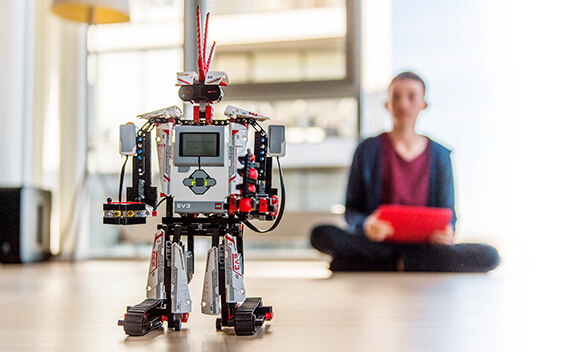
\includegraphics[width=0.5\textwidth]{figuras/lego_mindstorm.jpg}
    \caption[Caption for LOF]{Robot LEGO\textsuperscript{\textregistered} MINDSTORM\textsuperscript{\textregistered}}
    \label{fig:legomindstorm }
  \end{center}
\end{wrapfigure}

\subsection{Competencias especificas para el aprendizaje de un lenguaje de programación}

Para usar un lenguaje de programación (entendiendo este como un lenguaje formal de tipo especifico) como herramienta de enseñanza, es necesario tener en cuenta una serie de capacidades o características para que puedan ser incluidos en una currícula educativa. En general podemos decir que un lenguaje de programación debería tener las siguientes cualidades:

\begin{enumerate}
   \item Ser de alto nivel (similar a un lenguaje natural).
   \item Ser un lenguaje de propósito general (la capacidad de crear cualquier programa).
   \item Tener capacidad multi paradigma (programación orientada a objetos, programación estructurada, etc.).
   \item Ser multi plataforma (capacidad de adaptarse a distintos dispositivos).
 \end{enumerate} 
 
También, es importante que un lenguaje de programación seleccionado para trabajar en el aula sea de uso común y extendido en la industria, no tanto por su éxito comercial momentáneo, que puede variar en muy poco tiempo, si no por la capacidad de conseguir documentación especifica y comunidades de soporte que permitan desarrollar al máximo las capacidades intrínsecas de la herramienta.

Hay que hacer una aclaración respecto a los lenguajes de marcado (como HTML), que no son lenguajes de programación propiamente dicho dado que no tienen características básicas como:

\begin{itemize}
   \item variables
   \item repeticiones
   \item sentencias condicionales
   \item recursividad
 \end{itemize} 

Si bien esta enumeración de características no es exhaustiva, pone en manifiesto que, habiendo una enorme cantidad de lenguajes de programación, algunos de características mas especificas que otros, la elección del lenguaje de programación que se usará para un curso de enseñanza inicial no es un asunto trivial.


\section{Robótica y la enseñanza de programación}

En la actualidad, el uso de robótica se está extendiendo dentro de los espacios curriculares, los robots educativos se presentan como una alternativa interesante para poder trabajar conocimientos transversales a distintas disciplinas, desde la matemática y programación hasta las ciencias naturales. No obstante, se podría decir que dónde más se pueden aprovechar las ventajas de los kits de robótica que pululan en el mercado es precisamente en la enseñanza de los lenguajes de programación.

Básicamente un robot es una computadora con sensores y actuadores que le permiten interactuar en un entorno físico; para lograr ese cometido el robot debe ser programado con un algoritmo que le permita resolver las situaciones complejas que pueden ocurrir mientras se mueve por un medio ambiente físico. A diferencia de lo que ocurre en un entorno virtual como un simulador robótico, interactuar en un espacio físico obliga al diseñador del algoritmo a tomar medidas de corrección y control mediante sensores, y dotar al robot de cierta ''inteligencia'' para resolver situaciones inesperadas, como fallas mecánicas o defectos de fabricación. Esto ultimo sobre todo cuando se usan componentes reciclados o de baja calidad.

Es importante hacer una distinción entre ''aprendizaje DE robótica '' y ''aprendizaje CON robótica'' \citep{malec2001some}, entendiendo que la robótica es una disciplina en sí misma, y su uso en la industria tiene un nivel de complejidad que requiere un grado de especialización extra para los técnicos e ingenieros que trabajen en ese ámbito. Por eso mismo el aprendizaje CON robots, debería ser pensado como un medio para facilitar la construcción por parte de los discentes de conocimientos transversales adaptando las complejidades inherentes al diseño y construcción de un robot. Este aprendizaje CON  promueve en los estudiantes el desarrollo de competencias tales como: la toma de decisiones basadas en
el conocimiento, el formular explicaciones científicas y el trabajo en equipo \citep{lopez2013aprendizaje}.

\chapter{Proyecto educativo tecnológico}

\section{Introducción}

%\section{justificación}

%\section{objetivos}

%\section{metodologia}

%\section{capacitación}

%\section{duración}

%\section{gantt}

%\section{requerimientos}

%\section{herramientas para la construcción y mantenimiento de la plataforma}

%\section{componentes electro-mecanicos}

%\section{componentes electronicos}


%\cleardoublepage
\addcontentsline{toc}{chapter}{Referencias}
\bibliographystyle{apacite} % estilo de la bibliografía.
\bibliography{biblioteca/biblioteca_tesis} % yyyy.bib es el fichero donde está salvada la bibliografía.

\end{document}
